\documentclass[a4paper,ngerman,landscape]{scrartcl}

\usepackage[utf8]{inputenc}

\usepackage[ngerman]{babel}
\usepackage{hyperref}

\usepackage{graphicx}

\usepackage[protrusion=true,expansion=true]{microtype}

\usepackage{lmodern}
\usepackage{tabto}

\setlength\parskip{\medskipamount}
\setlength\parindent{0pt}

\usepackage{geometry}
\geometry{tmargin=0.5cm,bmargin=1.0cm,lmargin=2.5cm,rmargin=2.5cm}

\pagestyle{empty}

\begin{document}

\begin{center}
  \huge
  Freitag, 18. Oktober 2013, 14:00 Uhr, 2004/L1 \\
  \mbox{\textbf{Ingo Blechschmidt: Der Bohr-Topos}}
  \vfill
  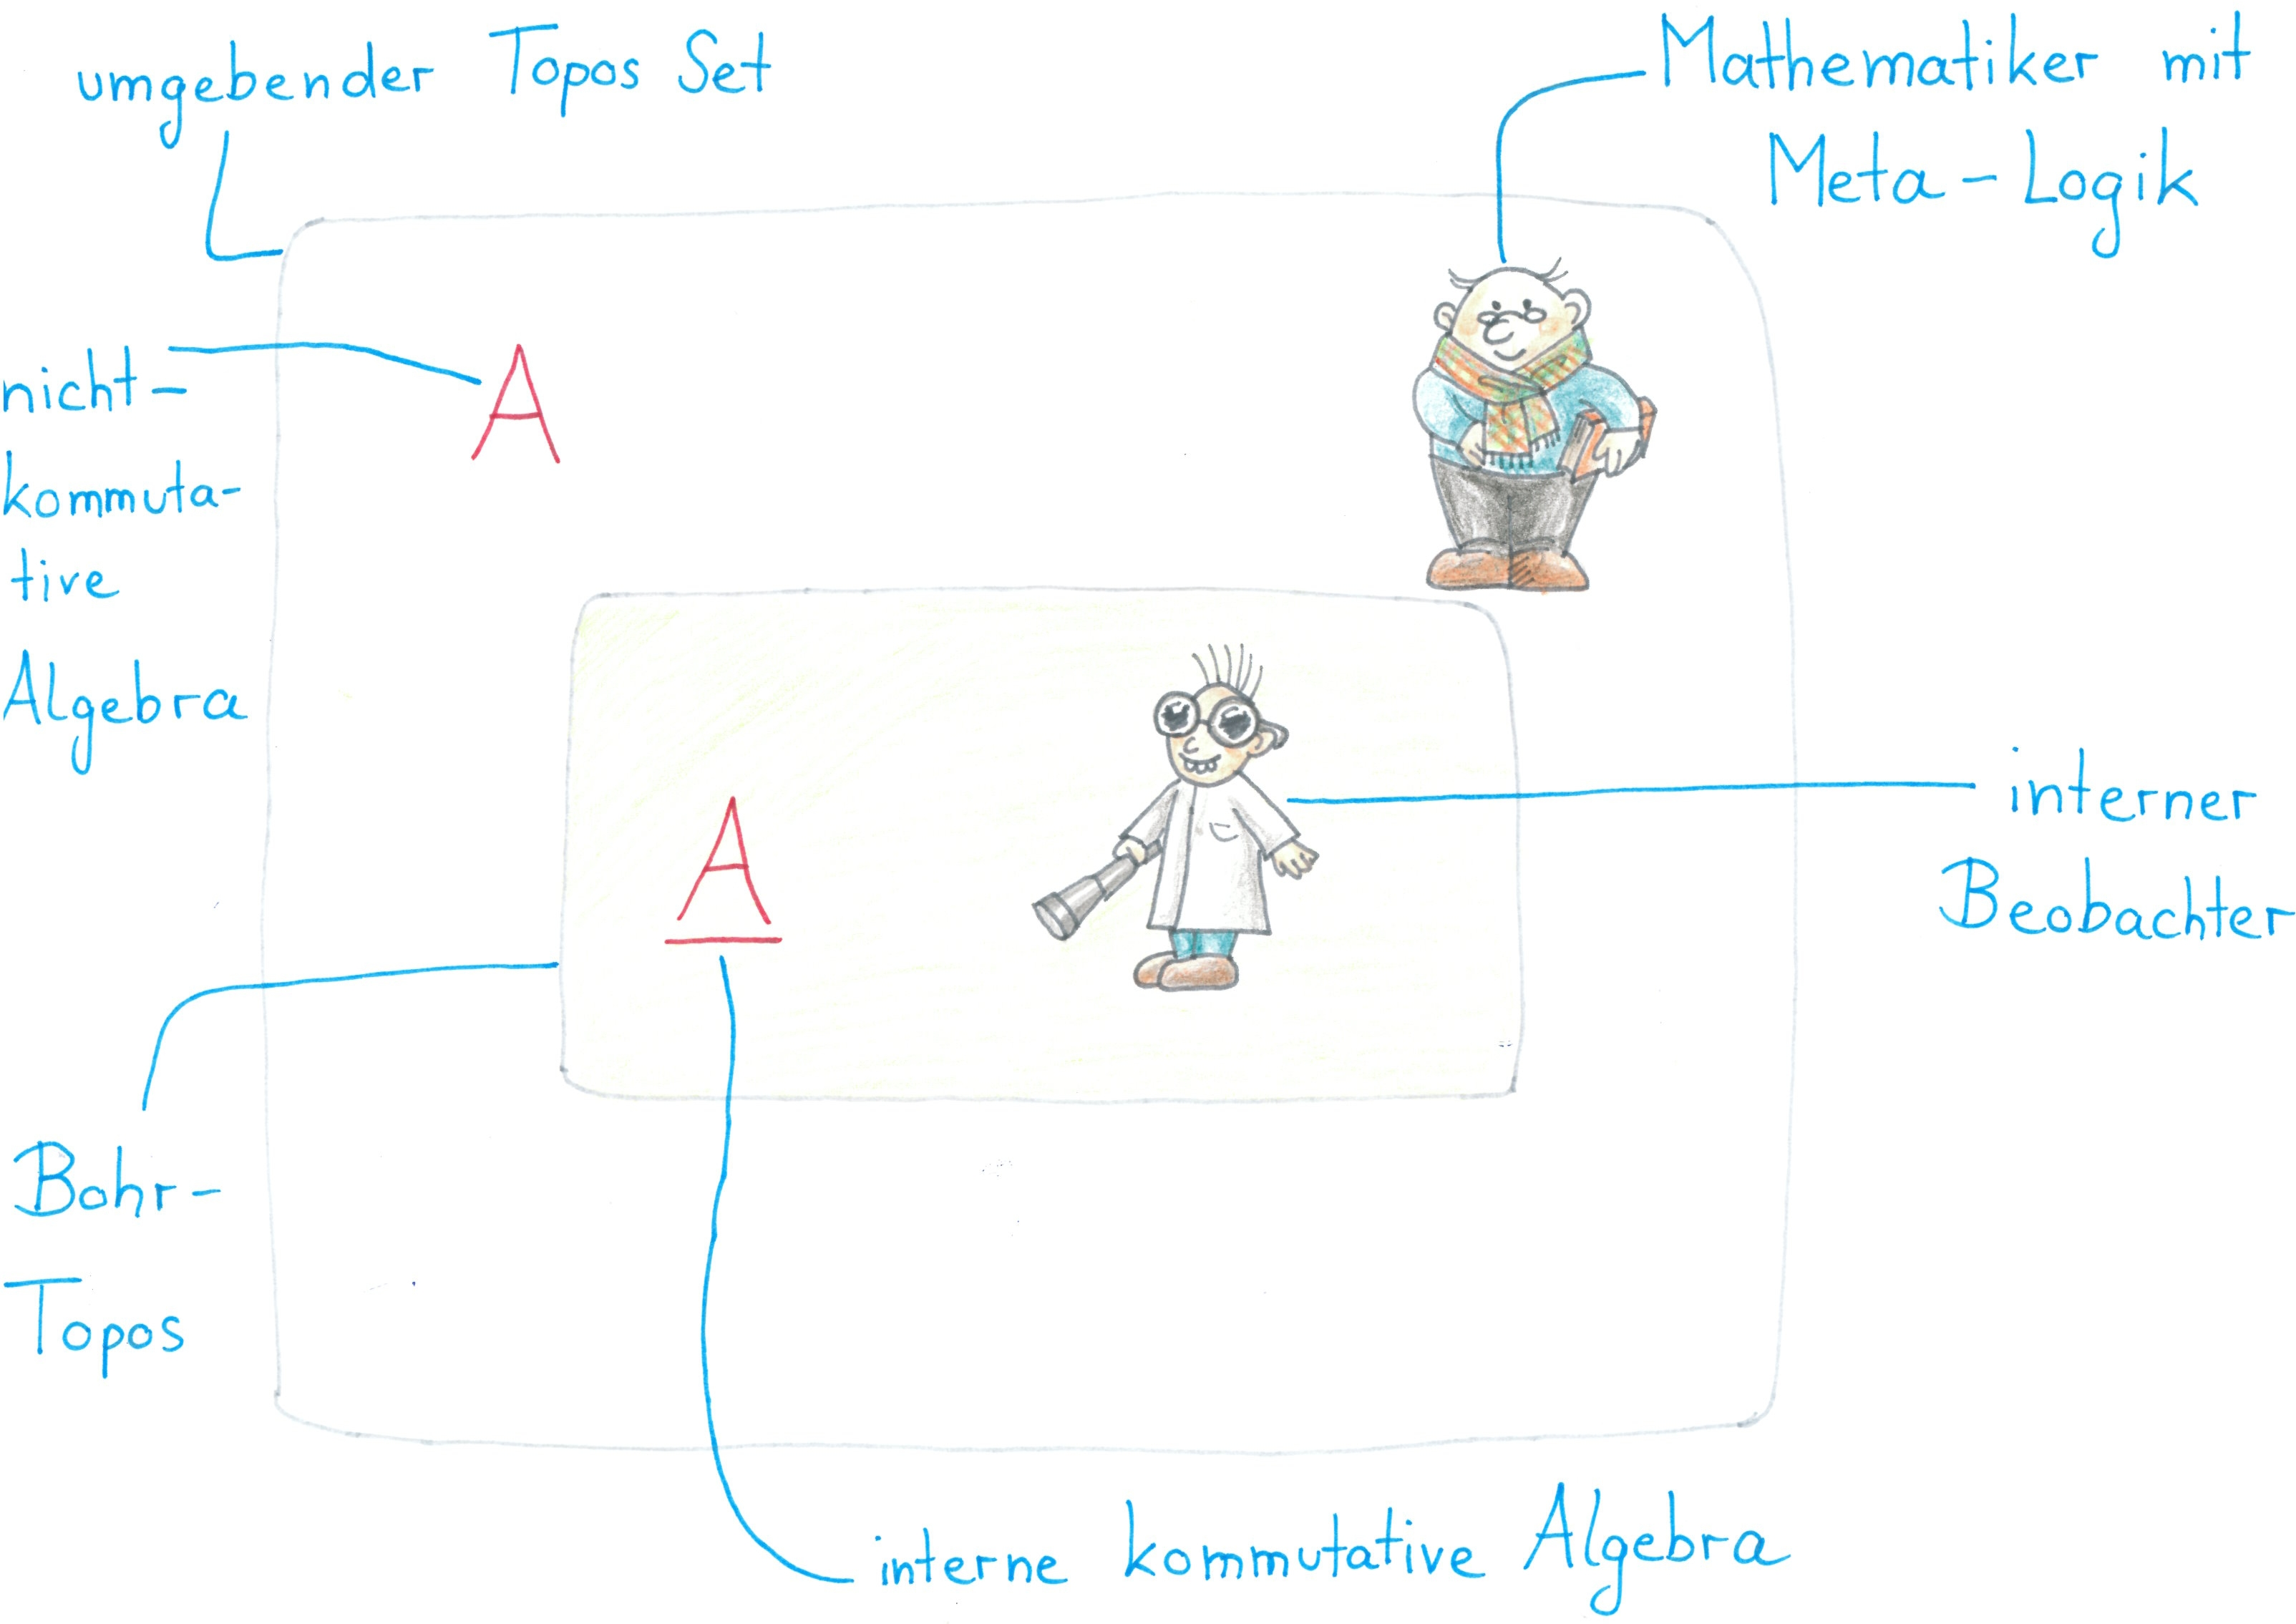
\includegraphics[scale=0.5]{bohr-topos}
  \vfill

  \large
  \begin{minipage}{0.8\textwidth}
    \setlength\parskip{\medskipamount}
    Die zu einem klassisch-mechanischen System gehörige~$C^\star$-Algebra ist
    kommutativ. Daher kann man ihr Gelfand-Spektrum betrachten; das ist ein
    topologischer Raum, der als Phasenraum für das untersuchte System fungiert.
    Die~$C^\star$-Algebra zu einem quantenmechanischen System ist dagegen
    nichtkommutativ; daher besitzt sie kein Gelfand-Spektrum und die schöne Idee
    eines Phasenraums ist nicht haltbar.

    Man kann aber den umgebenden Topos wechseln und die Situation aus der Sicht
    eines speziell an die nichtkommutative Algebra zugeschnittenen alternativen
    Mathematikuniversums betrachten, dem \emph{Bohr-Topos}.
    In dieser internen Sicht erscheint die Algebra kommutativ und
    besitzt somit wieder einen Phasenraum; in diesem (restriktiven) Sinn wird
    also Quantenmechanik bei interner Betrachtung zu klassischer Mechanik.

    Im Vortrag werden wir in einem groben und nicht-technischen Streifzug alle
    obigen Konzepte kennenlernen und auf dem Weg interessante Dinge wie
    mathematische Alternativuniversen und topologische Räume ohne Punkte
    mitnehmen. Wer nicht an physikalischen Anwendungen interessiert ist, kann
    daher trotzdem genug vom Vortrag mitnehmen, Voraussetzungen sind im
    Wesentlichen nur die Grundvorlesungen und nicht die vorherigen
    Pizzavorträge über konstruktive Mathematik.
  \end{minipage}
\end{center}

\newpage

\begin{center}
  \huge
  Freitag, 18. Oktober 2013, 15:45 Uhr, 2004/L1 \\
  \textbf{Sven Prüfer: Zöpfe}
  \vfill
  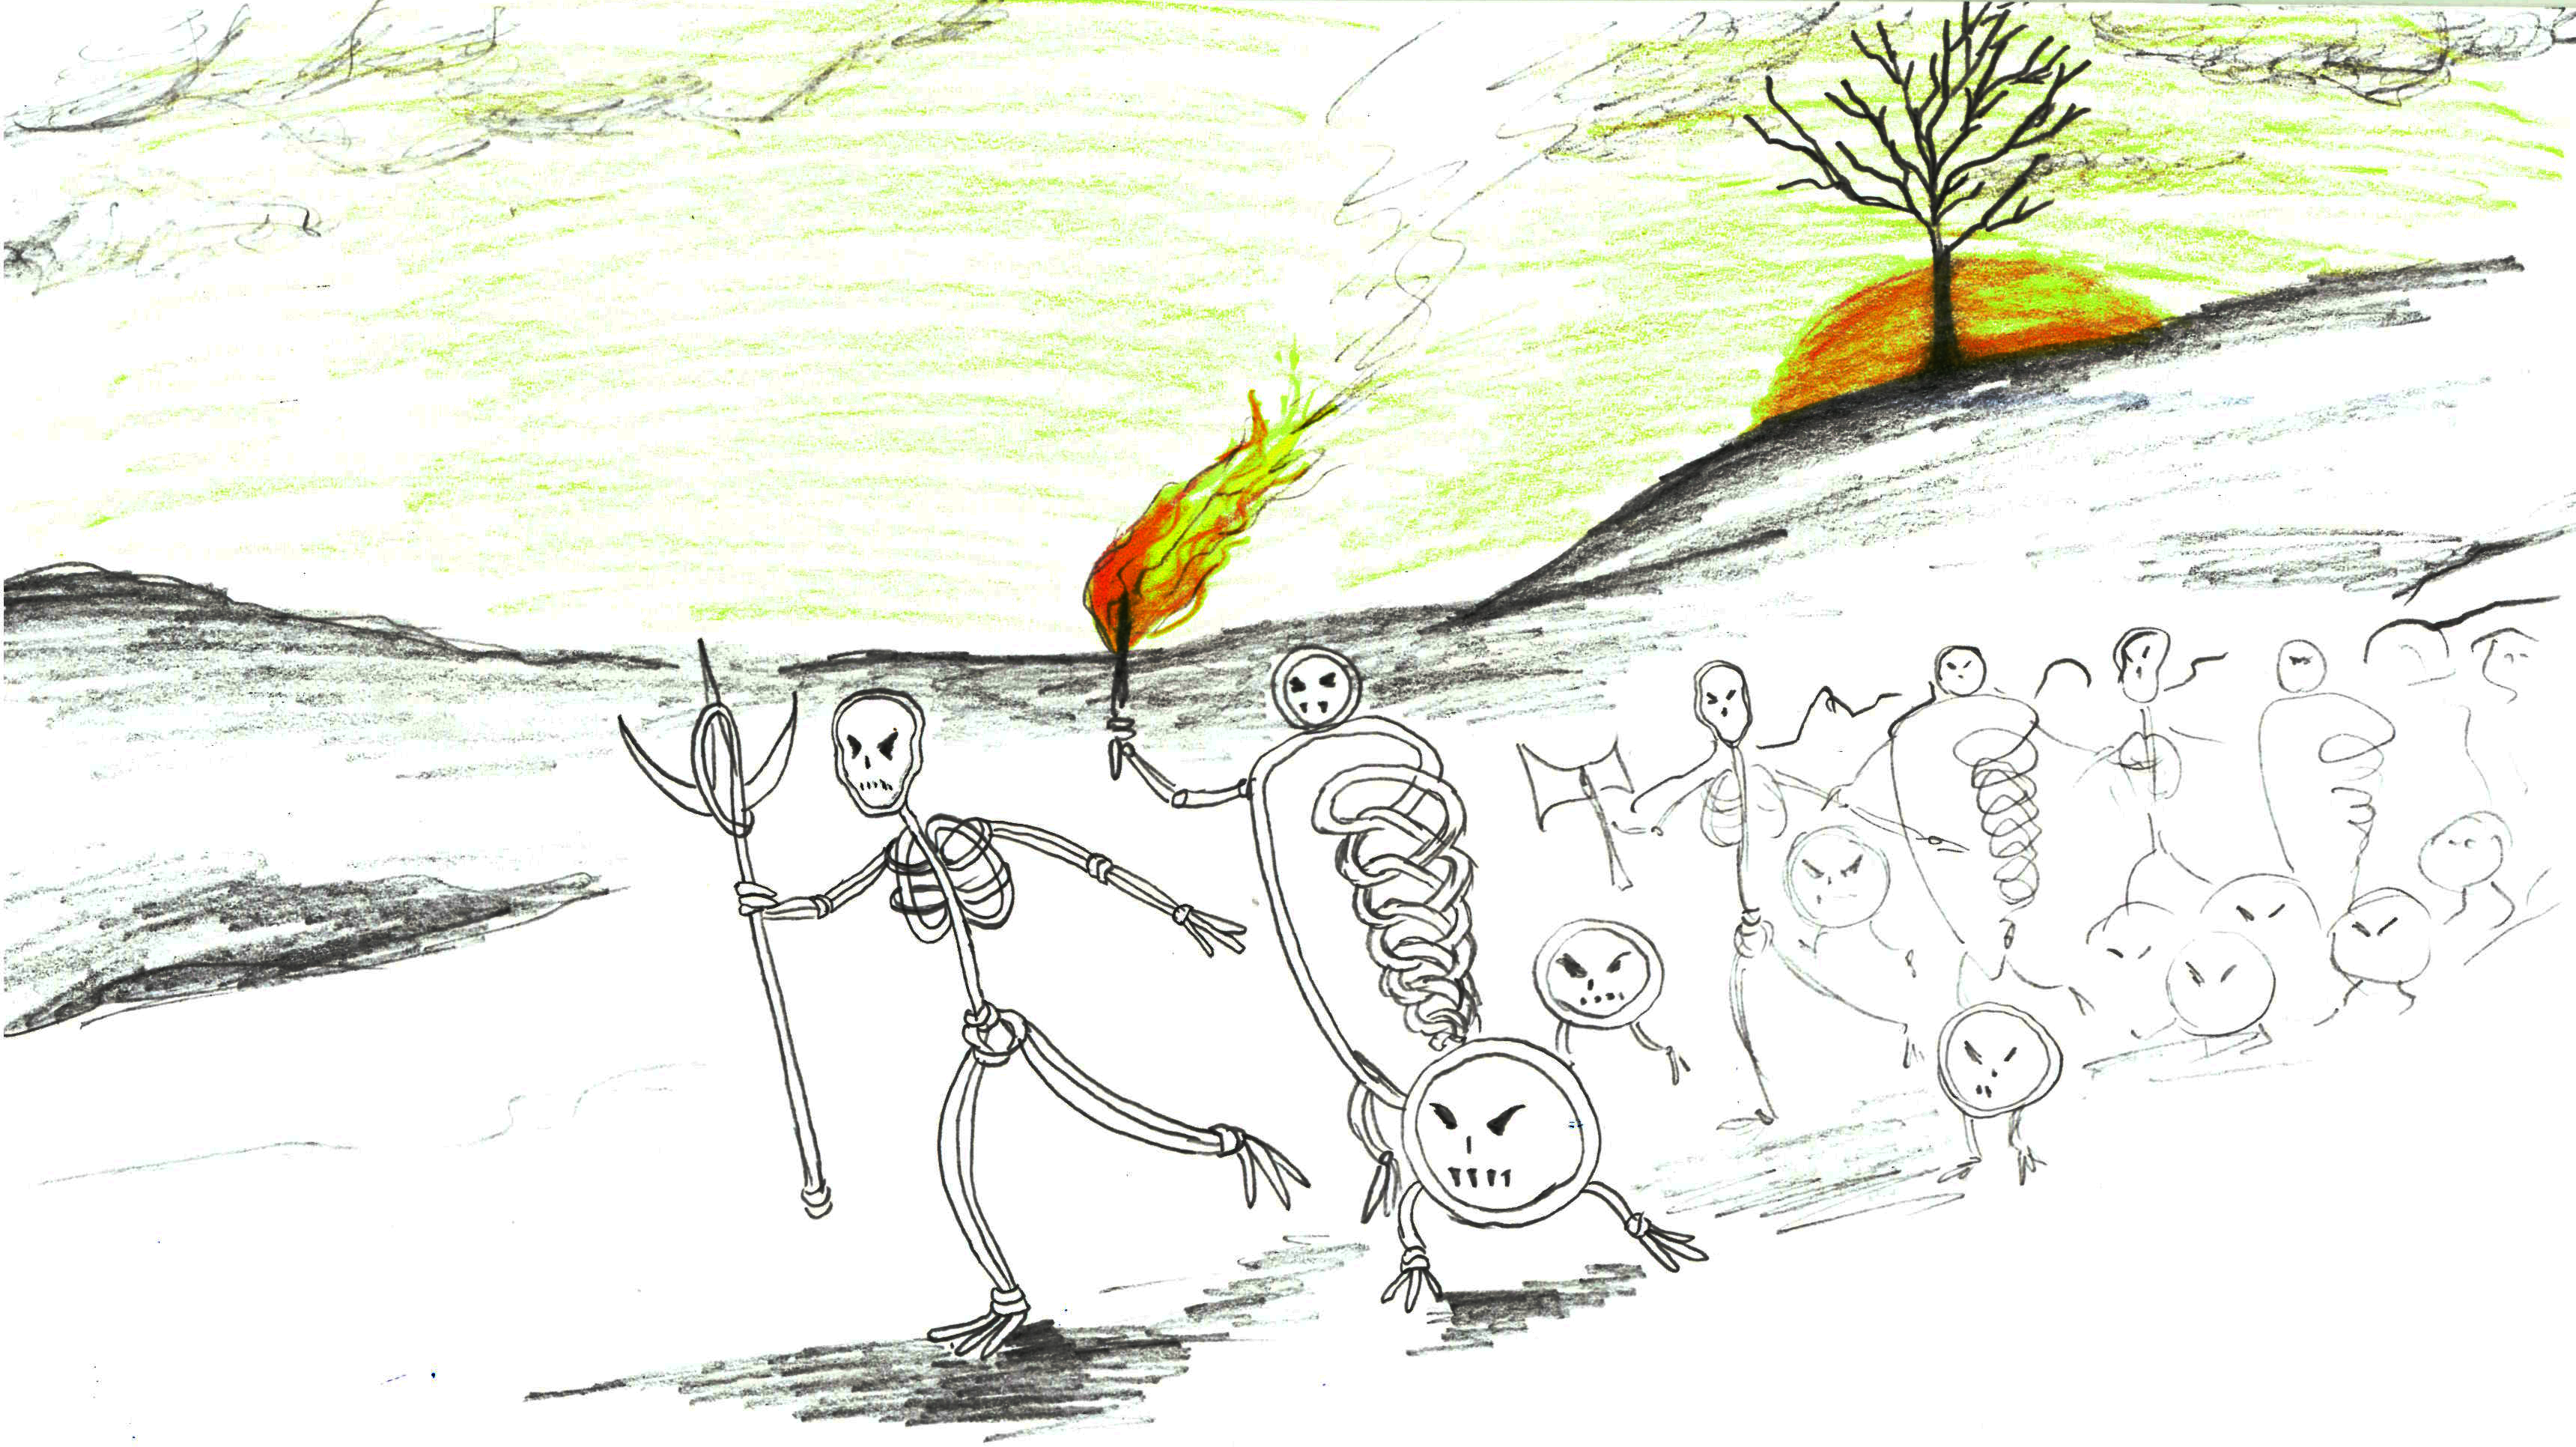
\includegraphics[scale=0.55]{knotenarmee-duester-farbkorrigiert}
  \vfill

  \large
  \begin{minipage}{0.8\textwidth}
    \setlength\parskip{\medskipamount}
    Zöpfe sind aufgeschnittene Knoten, sie bestehen also aus $n$~Strängen,
    welche~$n$ Anfangs- und Endpunkte verbinden. Wie bei den Knoten gibt es
    einen Isotopiebegriff. Der Vorteil ist, dass man Zöpfe
    verknüpfen kann und dadurch eine Gruppenstruktur erhält. Diese
    zusätzliche algebraische Struktur erlaubt wiederum andere Techniken aus
    der Trickkiste der Algebra zu nutzen. So lassen sich zum Beispiel viele
    Kno\-ten\-in\-va\-ri\-an\-ten durch geeignete Darstellungen der Zopfgruppe gewinnen.
    Außerdem kann man die Verzopfung auch in Kategorien betrachten.

    Im Vortrag werden zunächst geometrische Zöpfe und Zopfdiagramme
    definiert. Wir werden dann feststellen, dass die dadurch definierten
    Zopfgruppen isomorph zu den Artin-Zopfgruppen sind, für welche eine
    konkrete Präsentation mittels Erzeugern und Relationen existiert. Nach
    einer kurzen gruppentheoretischen Untersuchung wollen wir noch den Satz
    von Alexander verstehen, welcher besagt, dass jede Verschlingung isotop
    zu einem geschlossenen Zopf ist. Da alles sehr anschaulich ist, werden
    weder tiefere Vorkenntnisse aus der Mathematik noch Wissen aus den
    Knotentheorievorträgen benötigt. Alle Interessierten sind also herzlich
    eingeladen.
  \end{minipage}
\end{center}

\hfill\small Skript und Übungsblätter: \url{http://pizzaseminar.speicherleck.de/}
\end{document}
